\documentclass[twoside]{book}

% Packages required by doxygen
\usepackage{fixltx2e}
\usepackage{calc}
\usepackage{doxygen}
\usepackage[export]{adjustbox} % also loads graphicx
\usepackage{graphicx}
\usepackage[utf8]{inputenc}
\usepackage{makeidx}
\usepackage{multicol}
\usepackage{multirow}
\PassOptionsToPackage{warn}{textcomp}
\usepackage{textcomp}
\usepackage[nointegrals]{wasysym}
\usepackage[table]{xcolor}

% Font selection
\usepackage[T1]{fontenc}
\usepackage[scaled=.90]{helvet}
\usepackage{courier}
\usepackage{amssymb}
\usepackage{sectsty}
\renewcommand{\familydefault}{\sfdefault}
\allsectionsfont{%
  \fontseries{bc}\selectfont%
  \color{darkgray}%
}
\renewcommand{\DoxyLabelFont}{%
  \fontseries{bc}\selectfont%
  \color{darkgray}%
}
\newcommand{\+}{\discretionary{\mbox{\scriptsize$\hookleftarrow$}}{}{}}

% Page & text layout
\usepackage{geometry}
\geometry{%
  a4paper,%
  top=2.5cm,%
  bottom=2.5cm,%
  left=2.5cm,%
  right=2.5cm%
}
\tolerance=750
\hfuzz=15pt
\hbadness=750
\setlength{\emergencystretch}{15pt}
\setlength{\parindent}{0cm}
\setlength{\parskip}{3ex plus 2ex minus 2ex}
\makeatletter
\renewcommand{\paragraph}{%
  \@startsection{paragraph}{4}{0ex}{-1.0ex}{1.0ex}{%
    \normalfont\normalsize\bfseries\SS@parafont%
  }%
}
\renewcommand{\subparagraph}{%
  \@startsection{subparagraph}{5}{0ex}{-1.0ex}{1.0ex}{%
    \normalfont\normalsize\bfseries\SS@subparafont%
  }%
}
\makeatother

% Headers & footers
\usepackage{fancyhdr}
\pagestyle{fancyplain}
\fancyhead[LE]{\fancyplain{}{\bfseries\thepage}}
\fancyhead[CE]{\fancyplain{}{}}
\fancyhead[RE]{\fancyplain{}{\bfseries\leftmark}}
\fancyhead[LO]{\fancyplain{}{\bfseries\rightmark}}
\fancyhead[CO]{\fancyplain{}{}}
\fancyhead[RO]{\fancyplain{}{\bfseries\thepage}}
\fancyfoot[LE]{\fancyplain{}{}}
\fancyfoot[CE]{\fancyplain{}{}}
\fancyfoot[RE]{\fancyplain{}{\bfseries\scriptsize Generated by Doxygen }}
\fancyfoot[LO]{\fancyplain{}{\bfseries\scriptsize Generated by Doxygen }}
\fancyfoot[CO]{\fancyplain{}{}}
\fancyfoot[RO]{\fancyplain{}{}}
\renewcommand{\footrulewidth}{0.4pt}
\renewcommand{\chaptermark}[1]{%
  \markboth{#1}{}%
}
\renewcommand{\sectionmark}[1]{%
  \markright{\thesection\ #1}%
}

% Indices & bibliography
\usepackage{natbib}
\usepackage[titles]{tocloft}
\setcounter{tocdepth}{3}
\setcounter{secnumdepth}{5}
\makeindex

% Hyperlinks (required, but should be loaded last)
\usepackage{ifpdf}
\ifpdf
  \usepackage[pdftex,pagebackref=true]{hyperref}
\else
  \usepackage[ps2pdf,pagebackref=true]{hyperref}
\fi
\hypersetup{%
  colorlinks=true,%
  linkcolor=blue,%
  citecolor=blue,%
  unicode%
}

% Custom commands
\newcommand{\clearemptydoublepage}{%
  \newpage{\pagestyle{empty}\cleardoublepage}%
}

\usepackage{caption}
\captionsetup{labelsep=space,justification=centering,font={bf},singlelinecheck=off,skip=4pt,position=top}

%===== C O N T E N T S =====

\begin{document}

% Titlepage & ToC
\hypersetup{pageanchor=false,
             bookmarksnumbered=true,
             pdfencoding=unicode
            }
\pagenumbering{roman}
\begin{titlepage}
\vspace*{7cm}
\begin{center}%
{\Large Pepper\+\_\+walking \\[1ex]\large 0.\+1 }\\
\vspace*{1cm}
{\large Generated by Doxygen 1.8.11}\\
\end{center}
\end{titlepage}
\clearemptydoublepage
\tableofcontents
\clearemptydoublepage
\pagenumbering{arabic}
\hypersetup{pageanchor=true}

%--- Begin generated contents ---
\chapter{Class Index}
\section{Class List}
Here are the classes, structs, unions and interfaces with brief descriptions\+:\begin{DoxyCompactList}
\item\contentsline{section}{\hyperlink{classauto_walking}{auto\+Walking} }{\pageref{classauto_walking}}{}
\item\contentsline{section}{\hyperlink{classsensor_info}{sensor\+Info} }{\pageref{classsensor_info}}{}
\end{DoxyCompactList}

\chapter{File Index}
\section{File List}
Here is a list of all files with brief descriptions\+:\begin{DoxyCompactList}
\item\contentsline{section}{/home/mis/follow\+\_\+ws/src/pepper\+\_\+tracking/src/\hyperlink{asker_8cpp}{asker.\+cpp} \\*Do the bridge between the user ask and the image worker }{\pageref{asker_8cpp}}{}
\item\contentsline{section}{/home/mis/follow\+\_\+ws/src/pepper\+\_\+tracking/src/\hyperlink{worker_8cpp}{worker.\+cpp} \\*Do the bridge between visp, pepper and the user node }{\pageref{worker_8cpp}}{}
\end{DoxyCompactList}

\chapter{Class Documentation}
\hypertarget{classauto_walking}{}\section{auto\+Walking Class Reference}
\label{classauto_walking}\index{auto\+Walking@{auto\+Walking}}
\subsection*{Public Member Functions}
\begin{DoxyCompactItemize}
\item 
\hyperlink{classauto_walking_a6b81e2c604bbcf24bd34b5ddf7ea8270}{auto\+Walking} ()
\item 
void \hyperlink{classauto_walking_ae0f17930f80f5bf8e11bc246240b75a2}{Touch\+Head} (const std\+\_\+msgs\+::\+Int8 \&msg)
\begin{DoxyCompactList}\small\item\em Allow to have a sort of H\+IM on the head of Pepper. \end{DoxyCompactList}\item 
void \hyperlink{classauto_walking_a01b4702802806fc58ed344c226576535}{Front\+Distance} (const std\+\_\+msgs\+::\+Bool \&msg)
\begin{DoxyCompactList}\small\item\em Recup the front distance on the sonar. \end{DoxyCompactList}\item 
void \hyperlink{classauto_walking_a78e3b78ca7050490278b96474ffebb71}{Back\+Distance} (const std\+\_\+msgs\+::\+Bool \&msg)
\begin{DoxyCompactList}\small\item\em Recup the back distance on the sonar. \end{DoxyCompactList}\item 
void \hyperlink{classauto_walking_a383e14e4397ffeda34d43f9ebe94f52d}{Walking\+Call\+Back} (const ros\+::\+Timer\+Event \&event)
\begin{DoxyCompactList}\small\item\em Gesture of the possible movement, call each 0.\+1 seconde. \end{DoxyCompactList}\item 
void \hyperlink{classauto_walking_a38c0927b35e47c93d1d06ce57919f2e8}{Rotate\+Call\+Back} (const ros\+::\+Timer\+Event \&event)
\begin{DoxyCompactList}\small\item\em Find the better way to go after a stop. \end{DoxyCompactList}\item 
void \hyperlink{classauto_walking_add0dcc1657a0bc83fb487134883ca3de}{Stop\+Movement} ()
\begin{DoxyCompactList}\small\item\em Initialise and allow the programme to stop the movement. \end{DoxyCompactList}\item 
void \hyperlink{classauto_walking_a5eb7c4e92d91f27e830497c8ccfca973}{Go\+Forward} ()
\begin{DoxyCompactList}\small\item\em Initialise and allow the programme to go forward. \end{DoxyCompactList}\item 
void \hyperlink{classauto_walking_ab219370e461e832dafa9d3e48356f1b7}{Go\+Backward} ()
\begin{DoxyCompactList}\small\item\em Initialise and allow the programme to go backward. \end{DoxyCompactList}\end{DoxyCompactItemize}


\subsection{Detailed Description}


Definition at line 21 of file walking\+\_\+autonomous.\+cpp.



\subsection{Constructor \& Destructor Documentation}
\index{auto\+Walking@{auto\+Walking}!auto\+Walking@{auto\+Walking}}
\index{auto\+Walking@{auto\+Walking}!auto\+Walking@{auto\+Walking}}
\subsubsection[{\texorpdfstring{auto\+Walking()}{autoWalking()}}]{\setlength{\rightskip}{0pt plus 5cm}auto\+Walking\+::auto\+Walking (
\begin{DoxyParamCaption}
{}
\end{DoxyParamCaption}
)\hspace{0.3cm}{\ttfamily [inline]}}\hypertarget{classauto_walking_a6b81e2c604bbcf24bd34b5ddf7ea8270}{}\label{classauto_walking_a6b81e2c604bbcf24bd34b5ddf7ea8270}


Definition at line 24 of file walking\+\_\+autonomous.\+cpp.



\subsection{Member Function Documentation}
\index{auto\+Walking@{auto\+Walking}!Back\+Distance@{Back\+Distance}}
\index{Back\+Distance@{Back\+Distance}!auto\+Walking@{auto\+Walking}}
\subsubsection[{\texorpdfstring{Back\+Distance(const std\+\_\+msgs\+::\+Bool \&msg)}{BackDistance(const std_msgs::Bool &msg)}}]{\setlength{\rightskip}{0pt plus 5cm}void auto\+Walking\+::\+Back\+Distance (
\begin{DoxyParamCaption}
\item[{const std\+\_\+msgs\+::\+Bool \&}]{msg}
\end{DoxyParamCaption}
)\hspace{0.3cm}{\ttfamily [inline]}}\hypertarget{classauto_walking_a78e3b78ca7050490278b96474ffebb71}{}\label{classauto_walking_a78e3b78ca7050490278b96474ffebb71}


Recup the back distance on the sonar. 


\begin{DoxyParams}{Parameters}
{\em msg} & Input message from the Topic /demo\+\_\+control/sonar/back \\
\hline
\end{DoxyParams}
\begin{DoxyReturn}{Returns}
void 
\end{DoxyReturn}


Definition at line 101 of file walking\+\_\+autonomous.\+cpp.

\index{auto\+Walking@{auto\+Walking}!Front\+Distance@{Front\+Distance}}
\index{Front\+Distance@{Front\+Distance}!auto\+Walking@{auto\+Walking}}
\subsubsection[{\texorpdfstring{Front\+Distance(const std\+\_\+msgs\+::\+Bool \&msg)}{FrontDistance(const std_msgs::Bool &msg)}}]{\setlength{\rightskip}{0pt plus 5cm}void auto\+Walking\+::\+Front\+Distance (
\begin{DoxyParamCaption}
\item[{const std\+\_\+msgs\+::\+Bool \&}]{msg}
\end{DoxyParamCaption}
)\hspace{0.3cm}{\ttfamily [inline]}}\hypertarget{classauto_walking_a01b4702802806fc58ed344c226576535}{}\label{classauto_walking_a01b4702802806fc58ed344c226576535}


Recup the front distance on the sonar. 


\begin{DoxyParams}{Parameters}
{\em msg} & Input message from the Topic /demo\+\_\+control/sonar/front \\
\hline
\end{DoxyParams}
\begin{DoxyReturn}{Returns}
void 
\end{DoxyReturn}


Definition at line 90 of file walking\+\_\+autonomous.\+cpp.

\index{auto\+Walking@{auto\+Walking}!Go\+Backward@{Go\+Backward}}
\index{Go\+Backward@{Go\+Backward}!auto\+Walking@{auto\+Walking}}
\subsubsection[{\texorpdfstring{Go\+Backward()}{GoBackward()}}]{\setlength{\rightskip}{0pt plus 5cm}void auto\+Walking\+::\+Go\+Backward (
\begin{DoxyParamCaption}
{}
\end{DoxyParamCaption}
)\hspace{0.3cm}{\ttfamily [inline]}}\hypertarget{classauto_walking_ab219370e461e832dafa9d3e48356f1b7}{}\label{classauto_walking_ab219370e461e832dafa9d3e48356f1b7}


Initialise and allow the programme to go backward. 

\begin{DoxyReturn}{Returns}
void 
\end{DoxyReturn}


Definition at line 214 of file walking\+\_\+autonomous.\+cpp.

\index{auto\+Walking@{auto\+Walking}!Go\+Forward@{Go\+Forward}}
\index{Go\+Forward@{Go\+Forward}!auto\+Walking@{auto\+Walking}}
\subsubsection[{\texorpdfstring{Go\+Forward()}{GoForward()}}]{\setlength{\rightskip}{0pt plus 5cm}void auto\+Walking\+::\+Go\+Forward (
\begin{DoxyParamCaption}
{}
\end{DoxyParamCaption}
)\hspace{0.3cm}{\ttfamily [inline]}}\hypertarget{classauto_walking_a5eb7c4e92d91f27e830497c8ccfca973}{}\label{classauto_walking_a5eb7c4e92d91f27e830497c8ccfca973}


Initialise and allow the programme to go forward. 

\begin{DoxyReturn}{Returns}
void 
\end{DoxyReturn}


Definition at line 199 of file walking\+\_\+autonomous.\+cpp.

\index{auto\+Walking@{auto\+Walking}!Rotate\+Call\+Back@{Rotate\+Call\+Back}}
\index{Rotate\+Call\+Back@{Rotate\+Call\+Back}!auto\+Walking@{auto\+Walking}}
\subsubsection[{\texorpdfstring{Rotate\+Call\+Back(const ros\+::\+Timer\+Event \&event)}{RotateCallBack(const ros::TimerEvent &event)}}]{\setlength{\rightskip}{0pt plus 5cm}void auto\+Walking\+::\+Rotate\+Call\+Back (
\begin{DoxyParamCaption}
\item[{const ros\+::\+Timer\+Event \&}]{event}
\end{DoxyParamCaption}
)\hspace{0.3cm}{\ttfamily [inline]}}\hypertarget{classauto_walking_a38c0927b35e47c93d1d06ce57919f2e8}{}\label{classauto_walking_a38c0927b35e47c93d1d06ce57919f2e8}


Find the better way to go after a stop. 

evaluate obstacle at Left and Right with a cooldown of 10 secondes waiting until the rotation is finished


\begin{DoxyParams}{Parameters}
{\em event} & Necessary for the timer \\
\hline
\end{DoxyParams}
\begin{DoxyReturn}{Returns}
void 
\end{DoxyReturn}


Definition at line 148 of file walking\+\_\+autonomous.\+cpp.

\index{auto\+Walking@{auto\+Walking}!Stop\+Movement@{Stop\+Movement}}
\index{Stop\+Movement@{Stop\+Movement}!auto\+Walking@{auto\+Walking}}
\subsubsection[{\texorpdfstring{Stop\+Movement()}{StopMovement()}}]{\setlength{\rightskip}{0pt plus 5cm}void auto\+Walking\+::\+Stop\+Movement (
\begin{DoxyParamCaption}
{}
\end{DoxyParamCaption}
)\hspace{0.3cm}{\ttfamily [inline]}}\hypertarget{classauto_walking_add0dcc1657a0bc83fb487134883ca3de}{}\label{classauto_walking_add0dcc1657a0bc83fb487134883ca3de}


Initialise and allow the programme to stop the movement. 

\begin{DoxyReturn}{Returns}
void 
\end{DoxyReturn}


Definition at line 183 of file walking\+\_\+autonomous.\+cpp.

\index{auto\+Walking@{auto\+Walking}!Touch\+Head@{Touch\+Head}}
\index{Touch\+Head@{Touch\+Head}!auto\+Walking@{auto\+Walking}}
\subsubsection[{\texorpdfstring{Touch\+Head(const std\+\_\+msgs\+::\+Int8 \&msg)}{TouchHead(const std_msgs::Int8 &msg)}}]{\setlength{\rightskip}{0pt plus 5cm}void auto\+Walking\+::\+Touch\+Head (
\begin{DoxyParamCaption}
\item[{const std\+\_\+msgs\+::\+Int8 \&}]{msg}
\end{DoxyParamCaption}
)\hspace{0.3cm}{\ttfamily [inline]}}\hypertarget{classauto_walking_ae0f17930f80f5bf8e11bc246240b75a2}{}\label{classauto_walking_ae0f17930f80f5bf8e11bc246240b75a2}


Allow to have a sort of H\+IM on the head of Pepper. 

Subcriber Call\+Back


\begin{DoxyParams}{Parameters}
{\em msg} & Input message from the Topic /demo\+\_\+control/head\+\_\+touch \\
\hline
\end{DoxyParams}
\begin{DoxyReturn}{Returns}
void 
\end{DoxyReturn}


Definition at line 66 of file walking\+\_\+autonomous.\+cpp.

\index{auto\+Walking@{auto\+Walking}!Walking\+Call\+Back@{Walking\+Call\+Back}}
\index{Walking\+Call\+Back@{Walking\+Call\+Back}!auto\+Walking@{auto\+Walking}}
\subsubsection[{\texorpdfstring{Walking\+Call\+Back(const ros\+::\+Timer\+Event \&event)}{WalkingCallBack(const ros::TimerEvent &event)}}]{\setlength{\rightskip}{0pt plus 5cm}void auto\+Walking\+::\+Walking\+Call\+Back (
\begin{DoxyParamCaption}
\item[{const ros\+::\+Timer\+Event \&}]{event}
\end{DoxyParamCaption}
)\hspace{0.3cm}{\ttfamily [inline]}}\hypertarget{classauto_walking_a383e14e4397ffeda34d43f9ebe94f52d}{}\label{classauto_walking_a383e14e4397ffeda34d43f9ebe94f52d}


Gesture of the possible movement, call each 0.\+1 seconde. 

Timer Call\+Back

Go forward/backward if and while there are no obstacles Ask to find a new way when it\textquotesingle{}s blocked


\begin{DoxyParams}{Parameters}
{\em event} & Necessary for the timer \\
\hline
\end{DoxyParams}
\begin{DoxyReturn}{Returns}
void 
\end{DoxyReturn}


Definition at line 118 of file walking\+\_\+autonomous.\+cpp.



The documentation for this class was generated from the following file\+:\begin{DoxyCompactItemize}
\item 
/home/mis/follow\+\_\+ws/src/pepper\+\_\+walking/src/\hyperlink{walking__autonomous_8cpp}{walking\+\_\+autonomous.\+cpp}\end{DoxyCompactItemize}

\hypertarget{classsensor_info}{}\section{sensor\+Info Class Reference}
\label{classsensor_info}\index{sensor\+Info@{sensor\+Info}}
\subsection*{Public Member Functions}
\begin{DoxyCompactItemize}
\item 
\hyperlink{classsensor_info_a9a78f793919453ef7062a4be8dfc6693}{sensor\+Info} ()
\item 
void \hyperlink{classsensor_info_a3c05bf886c30bd9a58c267deac8a41c6}{touch\+Head} (const naoqi\+\_\+bridge\+\_\+msgs\+::\+Head\+Touch \&msg)
\begin{DoxyCompactList}\small\item\em Allow to have a sort of H\+IM on the head of Pepper. \end{DoxyCompactList}\item 
void \hyperlink{classsensor_info_a387ea702718ef6c83c4b8d34135d69dd}{sonar\+Front} (const sensor\+\_\+msgs\+::\+Range \&msg)
\begin{DoxyCompactList}\small\item\em Recup the front distance on the sonar. \end{DoxyCompactList}\item 
void \hyperlink{classsensor_info_aaa624fac38ad4a88acfa66f21a223238}{sonar\+Back} (const sensor\+\_\+msgs\+::\+Range \&msg)
\begin{DoxyCompactList}\small\item\em Recup the back distance on the sonar. \end{DoxyCompactList}\item 
void \hyperlink{classsensor_info_a0d8c9bb41d21a8d89330bd14fce5a6a2}{head\+Touch\+Call\+Back} (const ros\+::\+Timer\+Event \&event)
\begin{DoxyCompactList}\small\item\em Avoid to have too much messages on the pepper topic /speech. \end{DoxyCompactList}\item 
void \hyperlink{classsensor_info_a0a465025f366c28cce5d69da969e40e1}{sonar\+Front\+Call\+Back} (const ros\+::\+Timer\+Event \&event)
\item 
void \hyperlink{classsensor_info_a4f399406a35121ae1172d341e84c2531}{sonar\+Back\+Call\+Back} (const ros\+::\+Timer\+Event \&event)
\end{DoxyCompactItemize}


\subsection{Detailed Description}


Definition at line 22 of file walking\+\_\+sensor\+\_\+return.\+cpp.



\subsection{Constructor \& Destructor Documentation}
\index{sensor\+Info@{sensor\+Info}!sensor\+Info@{sensor\+Info}}
\index{sensor\+Info@{sensor\+Info}!sensor\+Info@{sensor\+Info}}
\subsubsection[{\texorpdfstring{sensor\+Info()}{sensorInfo()}}]{\setlength{\rightskip}{0pt plus 5cm}sensor\+Info\+::sensor\+Info (
\begin{DoxyParamCaption}
{}
\end{DoxyParamCaption}
)\hspace{0.3cm}{\ttfamily [inline]}}\hypertarget{classsensor_info_a9a78f793919453ef7062a4be8dfc6693}{}\label{classsensor_info_a9a78f793919453ef7062a4be8dfc6693}


Definition at line 25 of file walking\+\_\+sensor\+\_\+return.\+cpp.



\subsection{Member Function Documentation}
\index{sensor\+Info@{sensor\+Info}!head\+Touch\+Call\+Back@{head\+Touch\+Call\+Back}}
\index{head\+Touch\+Call\+Back@{head\+Touch\+Call\+Back}!sensor\+Info@{sensor\+Info}}
\subsubsection[{\texorpdfstring{head\+Touch\+Call\+Back(const ros\+::\+Timer\+Event \&event)}{headTouchCallBack(const ros::TimerEvent &event)}}]{\setlength{\rightskip}{0pt plus 5cm}void sensor\+Info\+::head\+Touch\+Call\+Back (
\begin{DoxyParamCaption}
\item[{const ros\+::\+Timer\+Event \&}]{event}
\end{DoxyParamCaption}
)\hspace{0.3cm}{\ttfamily [inline]}}\hypertarget{classsensor_info_a0d8c9bb41d21a8d89330bd14fce5a6a2}{}\label{classsensor_info_a0d8c9bb41d21a8d89330bd14fce5a6a2}


Avoid to have too much messages on the pepper topic /speech. 

Timer Call\+Back

Exe every seconde Say something when the head is touch


\begin{DoxyParams}{Parameters}
{\em event} & Necessary for the timer \\
\hline
\end{DoxyParams}
\begin{DoxyReturn}{Returns}
void
\end{DoxyReturn}
Exe every 3 seconde Say something if there\textquotesingle{}s an obstacle


\begin{DoxyParams}{Parameters}
{\em event} & Necessary for the timer \\
\hline
\end{DoxyParams}
\begin{DoxyReturn}{Returns}
void 
\end{DoxyReturn}


Definition at line 106 of file walking\+\_\+sensor\+\_\+return.\+cpp.

\index{sensor\+Info@{sensor\+Info}!sonar\+Back@{sonar\+Back}}
\index{sonar\+Back@{sonar\+Back}!sensor\+Info@{sensor\+Info}}
\subsubsection[{\texorpdfstring{sonar\+Back(const sensor\+\_\+msgs\+::\+Range \&msg)}{sonarBack(const sensor_msgs::Range &msg)}}]{\setlength{\rightskip}{0pt plus 5cm}void sensor\+Info\+::sonar\+Back (
\begin{DoxyParamCaption}
\item[{const sensor\+\_\+msgs\+::\+Range \&}]{msg}
\end{DoxyParamCaption}
)\hspace{0.3cm}{\ttfamily [inline]}}\hypertarget{classsensor_info_aaa624fac38ad4a88acfa66f21a223238}{}\label{classsensor_info_aaa624fac38ad4a88acfa66f21a223238}


Recup the back distance on the sonar. 


\begin{DoxyParams}{Parameters}
{\em msg} & Input message from the Topic /pepper\+\_\+robot/naoqi\+\_\+driver/sonar/back \\
\hline
\end{DoxyParams}
\begin{DoxyReturn}{Returns}
void 
\end{DoxyReturn}


Definition at line 87 of file walking\+\_\+sensor\+\_\+return.\+cpp.

\index{sensor\+Info@{sensor\+Info}!sonar\+Back\+Call\+Back@{sonar\+Back\+Call\+Back}}
\index{sonar\+Back\+Call\+Back@{sonar\+Back\+Call\+Back}!sensor\+Info@{sensor\+Info}}
\subsubsection[{\texorpdfstring{sonar\+Back\+Call\+Back(const ros\+::\+Timer\+Event \&event)}{sonarBackCallBack(const ros::TimerEvent &event)}}]{\setlength{\rightskip}{0pt plus 5cm}void sensor\+Info\+::sonar\+Back\+Call\+Back (
\begin{DoxyParamCaption}
\item[{const ros\+::\+Timer\+Event \&}]{event}
\end{DoxyParamCaption}
)\hspace{0.3cm}{\ttfamily [inline]}}\hypertarget{classsensor_info_a4f399406a35121ae1172d341e84c2531}{}\label{classsensor_info_a4f399406a35121ae1172d341e84c2531}


Definition at line 154 of file walking\+\_\+sensor\+\_\+return.\+cpp.

\index{sensor\+Info@{sensor\+Info}!sonar\+Front@{sonar\+Front}}
\index{sonar\+Front@{sonar\+Front}!sensor\+Info@{sensor\+Info}}
\subsubsection[{\texorpdfstring{sonar\+Front(const sensor\+\_\+msgs\+::\+Range \&msg)}{sonarFront(const sensor_msgs::Range &msg)}}]{\setlength{\rightskip}{0pt plus 5cm}void sensor\+Info\+::sonar\+Front (
\begin{DoxyParamCaption}
\item[{const sensor\+\_\+msgs\+::\+Range \&}]{msg}
\end{DoxyParamCaption}
)\hspace{0.3cm}{\ttfamily [inline]}}\hypertarget{classsensor_info_a387ea702718ef6c83c4b8d34135d69dd}{}\label{classsensor_info_a387ea702718ef6c83c4b8d34135d69dd}


Recup the front distance on the sonar. 


\begin{DoxyParams}{Parameters}
{\em msg} & Input message from the Topic /pepper\+\_\+robot/naoqi\+\_\+driver/sonar/front \\
\hline
\end{DoxyParams}
\begin{DoxyReturn}{Returns}
void 
\end{DoxyReturn}


Definition at line 73 of file walking\+\_\+sensor\+\_\+return.\+cpp.

\index{sensor\+Info@{sensor\+Info}!sonar\+Front\+Call\+Back@{sonar\+Front\+Call\+Back}}
\index{sonar\+Front\+Call\+Back@{sonar\+Front\+Call\+Back}!sensor\+Info@{sensor\+Info}}
\subsubsection[{\texorpdfstring{sonar\+Front\+Call\+Back(const ros\+::\+Timer\+Event \&event)}{sonarFrontCallBack(const ros::TimerEvent &event)}}]{\setlength{\rightskip}{0pt plus 5cm}void sensor\+Info\+::sonar\+Front\+Call\+Back (
\begin{DoxyParamCaption}
\item[{const ros\+::\+Timer\+Event \&}]{event}
\end{DoxyParamCaption}
)\hspace{0.3cm}{\ttfamily [inline]}}\hypertarget{classsensor_info_a0a465025f366c28cce5d69da969e40e1}{}\label{classsensor_info_a0a465025f366c28cce5d69da969e40e1}


Definition at line 132 of file walking\+\_\+sensor\+\_\+return.\+cpp.

\index{sensor\+Info@{sensor\+Info}!touch\+Head@{touch\+Head}}
\index{touch\+Head@{touch\+Head}!sensor\+Info@{sensor\+Info}}
\subsubsection[{\texorpdfstring{touch\+Head(const naoqi\+\_\+bridge\+\_\+msgs\+::\+Head\+Touch \&msg)}{touchHead(const naoqi_bridge_msgs::HeadTouch &msg)}}]{\setlength{\rightskip}{0pt plus 5cm}void sensor\+Info\+::touch\+Head (
\begin{DoxyParamCaption}
\item[{const naoqi\+\_\+bridge\+\_\+msgs\+::\+Head\+Touch \&}]{msg}
\end{DoxyParamCaption}
)\hspace{0.3cm}{\ttfamily [inline]}}\hypertarget{classsensor_info_a3c05bf886c30bd9a58c267deac8a41c6}{}\label{classsensor_info_a3c05bf886c30bd9a58c267deac8a41c6}


Allow to have a sort of H\+IM on the head of Pepper. 

Subcriber Call\+Back


\begin{DoxyParams}{Parameters}
{\em msg} & Input message from the Topic /pepper\+\_\+robot/naoqi\+\_\+driver/head\+\_\+touch \\
\hline
\end{DoxyParams}
\begin{DoxyReturn}{Returns}
void 
\end{DoxyReturn}


Definition at line 59 of file walking\+\_\+sensor\+\_\+return.\+cpp.



The documentation for this class was generated from the following file\+:\begin{DoxyCompactItemize}
\item 
/home/mis/follow\+\_\+ws/src/pepper\+\_\+walking/src/\hyperlink{walking__sensor__return_8cpp}{walking\+\_\+sensor\+\_\+return.\+cpp}\end{DoxyCompactItemize}

\chapter{File Documentation}
\hypertarget{walking__autonomous_8cpp}{}\section{/home/mis/follow\+\_\+ws/src/pepper\+\_\+walking/src/walking\+\_\+autonomous.cpp File Reference}
\label{walking__autonomous_8cpp}\index{/home/mis/follow\+\_\+ws/src/pepper\+\_\+walking/src/walking\+\_\+autonomous.\+cpp@{/home/mis/follow\+\_\+ws/src/pepper\+\_\+walking/src/walking\+\_\+autonomous.\+cpp}}


Subcribe, analyse and convert all the data of the sonar and head topics.  


{\ttfamily \#include $<$ros/ros.\+h$>$}\\*
{\ttfamily \#include $<$std\+\_\+msgs/\+Int8.\+h$>$}\\*
{\ttfamily \#include $<$std\+\_\+msgs/\+Bool.\+h$>$}\\*
{\ttfamily \#include $<$geometry\+\_\+msgs/\+Twist.\+h$>$}\\*
{\ttfamily \#include $<$geometry\+\_\+msgs/\+Pose\+Stamped.\+h$>$}\\*
{\ttfamily \#include $<$time.\+h$>$}\\*
Include dependency graph for walking\+\_\+autonomous.\+cpp\+:
\nopagebreak
\begin{figure}[H]
\begin{center}
\leavevmode
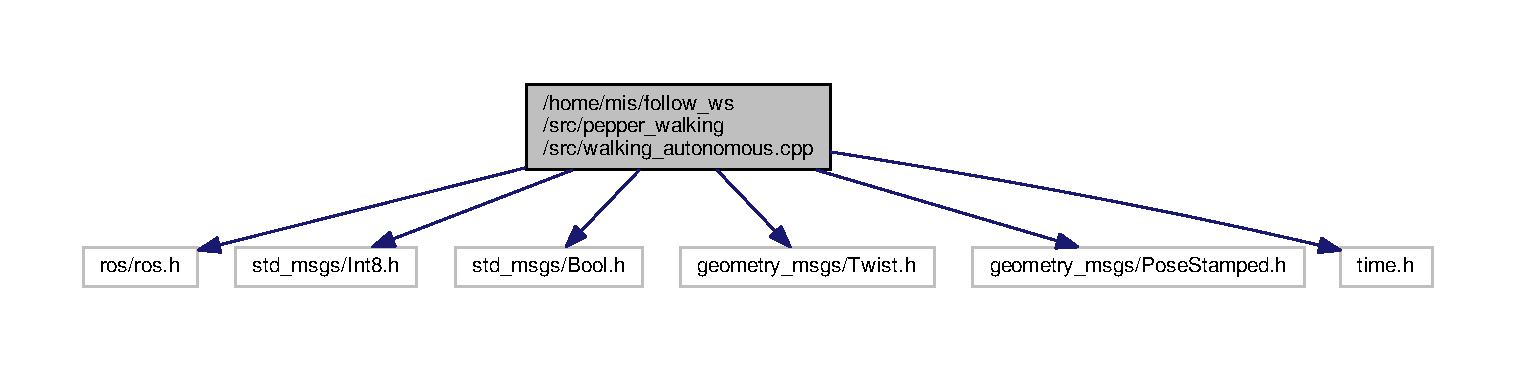
\includegraphics[width=350pt]{walking__autonomous_8cpp__incl}
\end{center}
\end{figure}
\subsection*{Classes}
\begin{DoxyCompactItemize}
\item 
class \hyperlink{classauto_walking}{auto\+Walking}
\end{DoxyCompactItemize}
\subsection*{Functions}
\begin{DoxyCompactItemize}
\item 
int \hyperlink{walking__autonomous_8cpp_a3c04138a5bfe5d72780bb7e82a18e627}{main} (int argc, char $\ast$$\ast$argv)
\end{DoxyCompactItemize}


\subsection{Detailed Description}
Subcribe, analyse and convert all the data of the sonar and head topics. 

\begin{DoxyAuthor}{Author}
Vivien.\+C 
\end{DoxyAuthor}
\begin{DoxyDate}{Date}
02/05/2018
\end{DoxyDate}
Convert distance from sonar to a simple data Use head of Pepper like an interface with human Say somes things during some actions or evenements 

\subsection{Function Documentation}
\index{walking\+\_\+autonomous.\+cpp@{walking\+\_\+autonomous.\+cpp}!main@{main}}
\index{main@{main}!walking\+\_\+autonomous.\+cpp@{walking\+\_\+autonomous.\+cpp}}
\subsubsection[{\texorpdfstring{main(int argc, char $\ast$$\ast$argv)}{main(int argc, char **argv)}}]{\setlength{\rightskip}{0pt plus 5cm}int main (
\begin{DoxyParamCaption}
\item[{int}]{argc, }
\item[{char $\ast$$\ast$}]{argv}
\end{DoxyParamCaption}
)}\hypertarget{walking__autonomous_8cpp_a3c04138a5bfe5d72780bb7e82a18e627}{}\label{walking__autonomous_8cpp_a3c04138a5bfe5d72780bb7e82a18e627}


Definition at line 242 of file walking\+\_\+autonomous.\+cpp.


\hypertarget{walking__sensor__return_8cpp}{}\section{/home/mis/follow\+\_\+ws/src/pepper\+\_\+walking/src/walking\+\_\+sensor\+\_\+return.cpp File Reference}
\label{walking__sensor__return_8cpp}\index{/home/mis/follow\+\_\+ws/src/pepper\+\_\+walking/src/walking\+\_\+sensor\+\_\+return.\+cpp@{/home/mis/follow\+\_\+ws/src/pepper\+\_\+walking/src/walking\+\_\+sensor\+\_\+return.\+cpp}}
{\ttfamily \#include $<$ros/ros.\+h$>$}\\*
{\ttfamily \#include $<$string$>$}\\*
{\ttfamily \#include $<$naoqi\+\_\+bridge\+\_\+msgs/\+Head\+Touch.\+h$>$}\\*
{\ttfamily \#include $<$sensor\+\_\+msgs/\+Range.\+h$>$}\\*
{\ttfamily \#include $<$std\+\_\+msgs/\+Int8.\+h$>$}\\*
{\ttfamily \#include $<$std\+\_\+msgs/\+String.\+h$>$}\\*
{\ttfamily \#include $<$std\+\_\+msgs/\+Bool.\+h$>$}\\*
Include dependency graph for walking\+\_\+sensor\+\_\+return.\+cpp\+:
\nopagebreak
\begin{figure}[H]
\begin{center}
\leavevmode
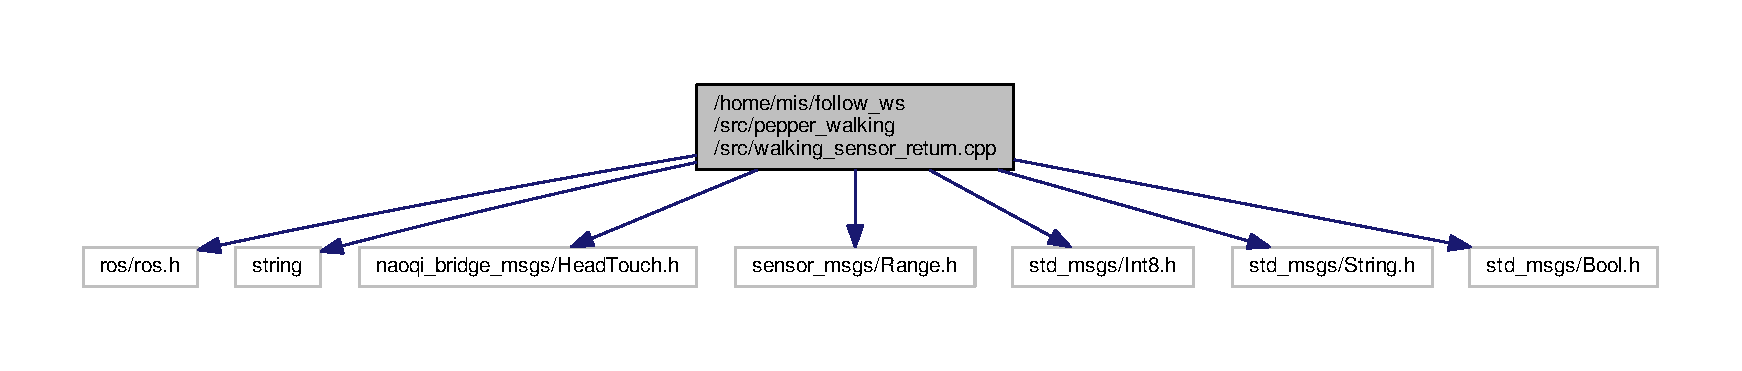
\includegraphics[width=350pt]{walking__sensor__return_8cpp__incl}
\end{center}
\end{figure}
\subsection*{Classes}
\begin{DoxyCompactItemize}
\item 
class \hyperlink{classsensor_info}{sensor\+Info}
\end{DoxyCompactItemize}
\subsection*{Functions}
\begin{DoxyCompactItemize}
\item 
int \hyperlink{walking__sensor__return_8cpp_a3c04138a5bfe5d72780bb7e82a18e627}{main} (int argc, char $\ast$$\ast$argv)
\end{DoxyCompactItemize}


\subsection{Function Documentation}
\index{walking\+\_\+sensor\+\_\+return.\+cpp@{walking\+\_\+sensor\+\_\+return.\+cpp}!main@{main}}
\index{main@{main}!walking\+\_\+sensor\+\_\+return.\+cpp@{walking\+\_\+sensor\+\_\+return.\+cpp}}
\subsubsection[{\texorpdfstring{main(int argc, char $\ast$$\ast$argv)}{main(int argc, char **argv)}}]{\setlength{\rightskip}{0pt plus 5cm}int main (
\begin{DoxyParamCaption}
\item[{int}]{argc, }
\item[{char $\ast$$\ast$}]{argv}
\end{DoxyParamCaption}
)}\hypertarget{walking__sensor__return_8cpp_a3c04138a5bfe5d72780bb7e82a18e627}{}\label{walking__sensor__return_8cpp_a3c04138a5bfe5d72780bb7e82a18e627}


Definition at line 183 of file walking\+\_\+sensor\+\_\+return.\+cpp.


%--- End generated contents ---

% Index
\backmatter
\newpage
\phantomsection
\clearemptydoublepage
\addcontentsline{toc}{chapter}{Index}
\printindex

\end{document}
